%% Supplementary material for: Machine Learning Models for Mental-Health Prediction from Actigraphy:
%% A Systematic Appraisal and an Empirical Demonstration. Standalone; compile with pdflatex.
\documentclass[11pt,a4paper]{article}
\usepackage[T1]{fontenc}\usepackage[utf8]{inputenc}\usepackage{lmodern}\usepackage{microtype}
\usepackage[margin=2.3cm]{geometry}\usepackage{booktabs}\usepackage{graphicx}\usepackage{longtable}
\usepackage{amsmath}\usepackage{array}\usepackage{xcolor}\usepackage{adjustbox}\usepackage[hidelinks]{hyperref}
\graphicspath{{../empirical/figures/}{figures/}}
\renewcommand{\thetable}{S\arabic{table}}\renewcommand{\thefigure}{S\arabic{figure}}
\setlength{\parskip}{0.35em}\setlength{\parindent}{0pt}
\title{Supplementary material\\[0.3em]\large Machine Learning Models for Mental-Health Prediction from Actigraphy:\\A Systematic Appraisal and an Empirical Demonstration}
\author{Aminat Abiola Ajibola$^{1,*}$ \and Roger Nick Anaedevha$^{2}$}
\date{\footnotesize $^{1}$College of Computer Science and Engineering, University of Hafr Al-Batin, Eastern Province, Kingdom of Saudi Arabia\\
$^{2}$Institute of Cyber Intelligence Systems, National Research Nuclear University MEPhI, Moscow, Russian Federation\\
$^{*}$aajibola@uhb.edu.sa \quad Code and results: \url{https://github.com/rogerpanel/cv/tree/main/mlmh-appraisal}}
\begin{document}
\maketitle
\tableofcontents

\section{Table S1: TRIPOD+AI checklist}
The checklist follows Collins et al.\ (BMJ 2024;385:e078378). Item numbering follows the
extraction workbook used in Part~I; section references are to the main article.
\input{supplement_tripod_checklist}

\section{Table S2: feature definitions}
\input{supplement_features}

\section{Tables S3 and S4: identification sources and study list for Part I}
\input{supplement_part1_sources}

\section{Table S5: run manifests and prediction files}
Every experiment run writes \path{results/real/<experiment>/manifest.json} with the fields in
Table~\ref{tab:manifest}, and every model--splitter combination writes its out-of-fold predictions
to \path{results/real/<experiment>/predictions/<cohort>.<model>.<splitter>.csv} with one row per
seed, fold and day window (columns: seed, fold, window\_id, subject\_id, cohort, y, p). The tables
in the main article are regenerated from these files by \path{python -m mlmh retable} and
\path{scripts/update_readme.py}; the Part~I figure and table by \path{scripts/part1_figure.py};
the calibration and radar figures and the comparison table by \path{scripts/part2_extra_figures.py}.
\begin{table}[!htbp]\centering\caption{Fields of a run manifest.}\label{tab:manifest}\footnotesize
\begin{tabular}{ll}\toprule Field & Content\\\midrule
created\_utc & Timestamp of the run\\
git\_sha, git\_dirty & Commit of the code that produced the run; whether the tree had uncommitted changes\\
config\_hash, config & SHA-256 prefix of the resolved configuration and the configuration itself (seeds, folds, models, bootstrap)\\
python, platform, package\_versions & Interpreter, OS, and versions of numpy, pandas, scikit-learn, xgboost, imbalanced-learn, scipy, matplotlib, torch\\
dataset\_checksums & SHA-256 of every raw CSV file of every cohort used\\
synthetic & Whether the run used the synthetic fixture (always false for reported results)\\
experiment, n\_rows & Experiment name and number of result rows written\\
\bottomrule\end{tabular}\end{table}

\section{Figures S1 to S3: ROC and reliability curves}
\begin{figure}[!htbp]\centering
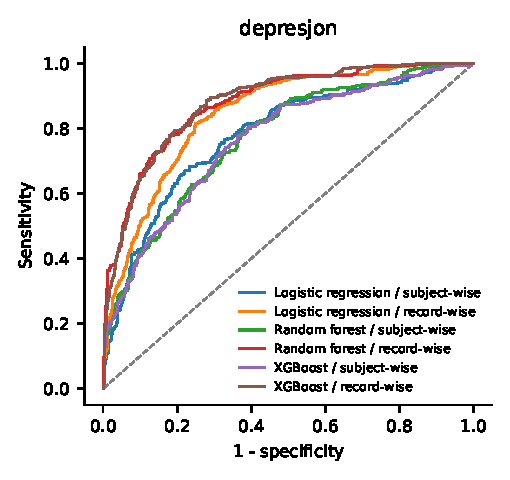
\includegraphics[width=.32\linewidth]{e1_roc_depresjon.pdf}\hfill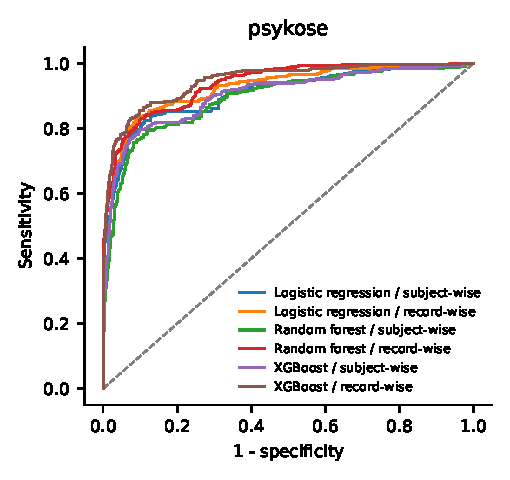
\includegraphics[width=.32\linewidth]{e1_roc_psykose.pdf}\hfill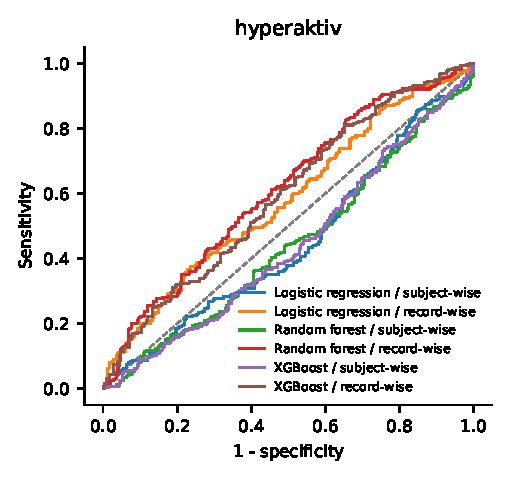
\includegraphics[width=.32\linewidth]{e1_roc_hyperaktiv.pdf}\\[0.4em]
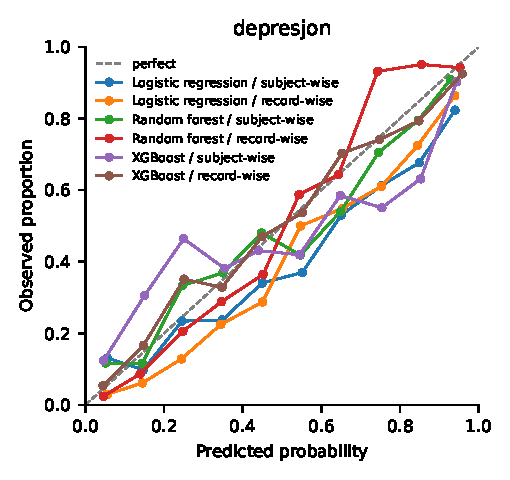
\includegraphics[width=.32\linewidth]{e1_reliability_depresjon.pdf}\hfill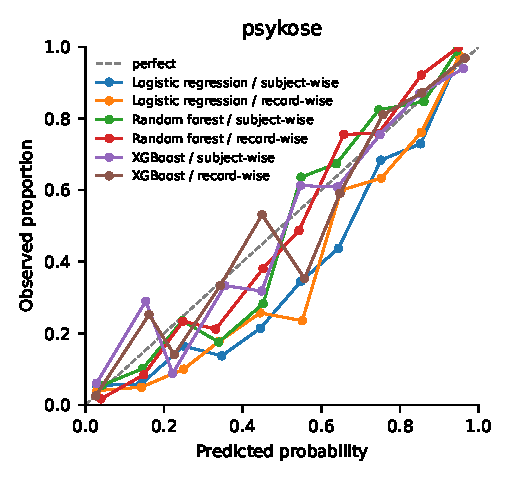
\includegraphics[width=.32\linewidth]{e1_reliability_psykose.pdf}\hfill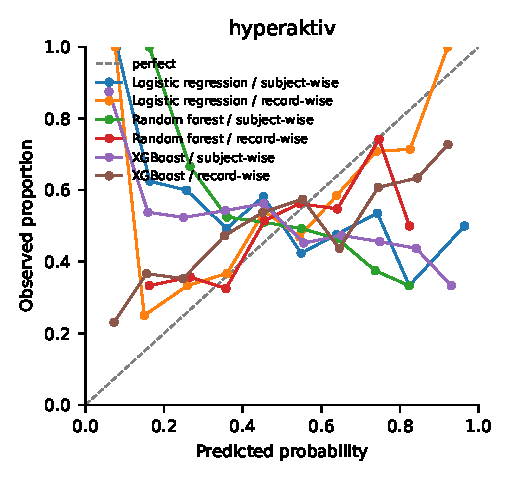
\includegraphics[width=.32\linewidth]{e1_reliability_hyperaktiv.pdf}
\caption{E1. ROC (top) and reliability (bottom) curves of the seed-averaged out-of-fold predictions for every model under subject-wise and record-wise cross-validation, per cohort.}\end{figure}
\begin{figure}[!htbp]\centering
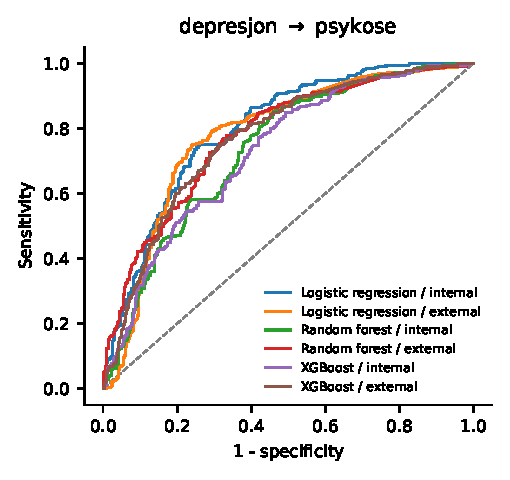
\includegraphics[width=.32\linewidth]{e2_roc_depresjon_to_psykose.pdf}\hfill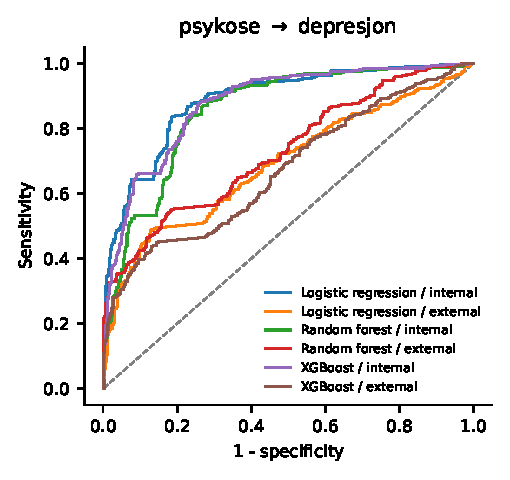
\includegraphics[width=.32\linewidth]{e2_roc_psykose_to_depresjon.pdf}\hfill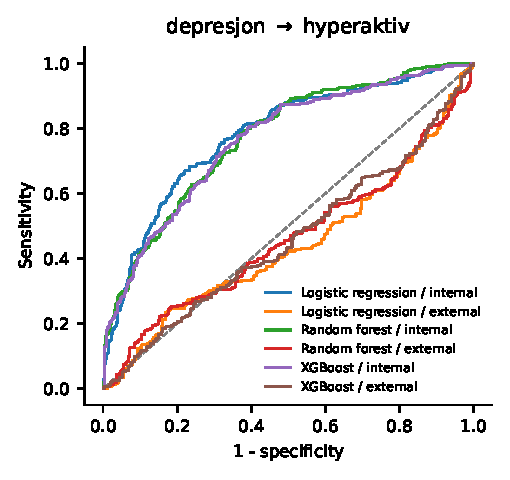
\includegraphics[width=.32\linewidth]{e2_roc_depresjon_to_hyperaktiv.pdf}\\[0.4em]
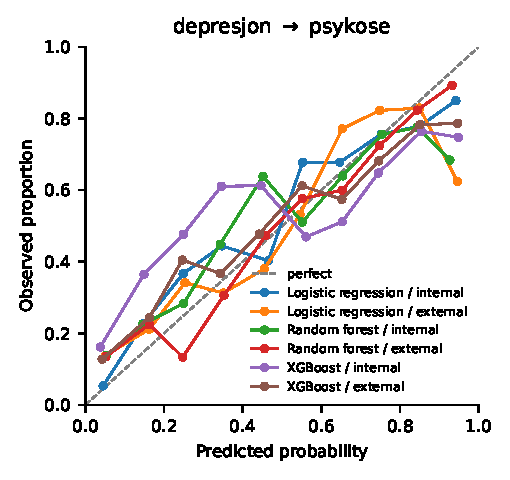
\includegraphics[width=.32\linewidth]{e2_reliability_depresjon_to_psykose.pdf}\hfill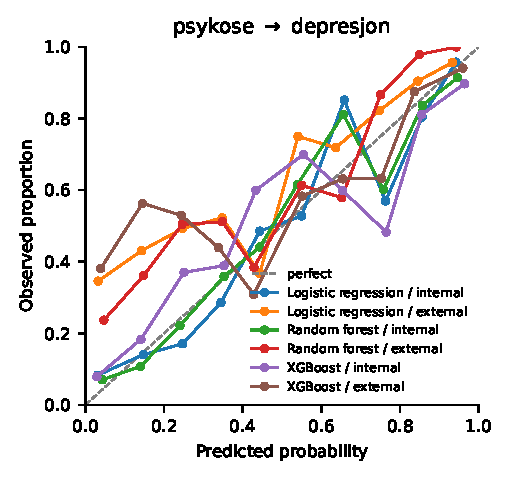
\includegraphics[width=.32\linewidth]{e2_reliability_psykose_to_depresjon.pdf}\hfill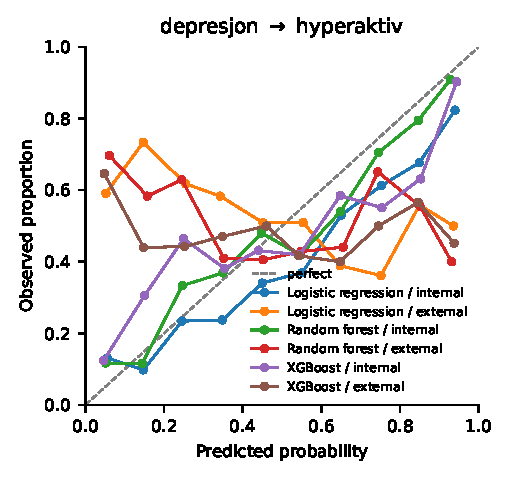
\includegraphics[width=.32\linewidth]{e2_reliability_depresjon_to_hyperaktiv.pdf}
\caption{E2. ROC (top) and reliability (bottom) curves of internal (subject-wise CV on the training cohort) and external (frozen model on the test cohort) predictions for each cohort pair.}\end{figure}
\begin{figure}[!htbp]\centering
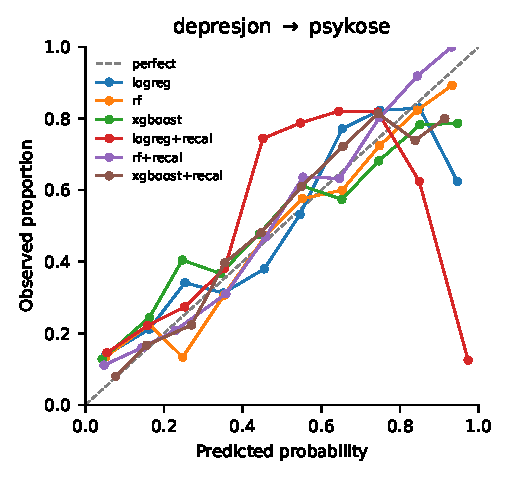
\includegraphics[width=.32\linewidth]{e3_reliability_depresjon_to_psykose.pdf}\hfill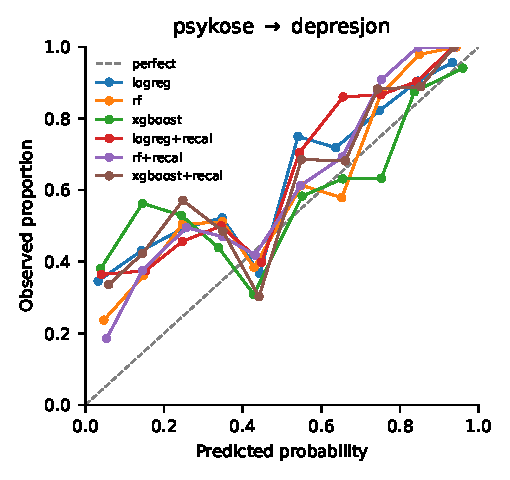
\includegraphics[width=.32\linewidth]{e3_reliability_psykose_to_depresjon.pdf}\hfill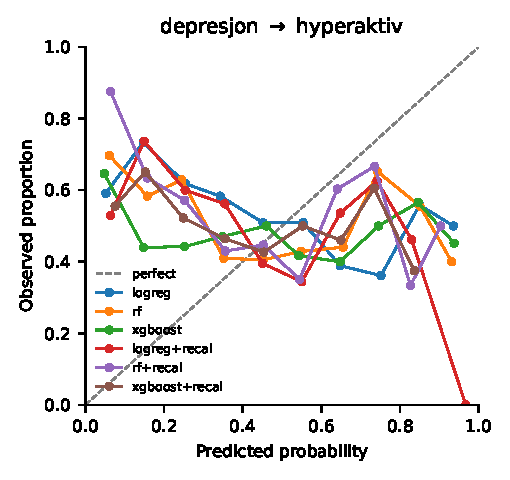
\includegraphics[width=.32\linewidth]{e3_reliability_depresjon_to_hyperaktiv.pdf}
\caption{E3. Reliability curves of external predictions before and after logistic recalibration fitted on the training cohort's out-of-fold predictions, per cohort pair.}\end{figure}
\end{document}
